\documentclass[12pt,oneside]{report}
\usepackage{xcolor}
\usepackage{tikz}
\usetikzlibrary{calc}
\usepackage{multicol}
\usepackage{titletoc}
\usepackage{ragged2e}
\usepackage{fancyhdr} 
\usepackage{url}
\usepackage{verbatim}
\usepackage[utf8]{inputenc}
\usepackage[bookmarks, colorlinks=false, pdfborder={0 0 0}, pdftitle={<pdf title here>}, pdfauthor={<author's name here>}, pdfsubject={<subject here>}, pdfkeywords={<keywords here>}]{hyperref} 

\usepackage{etoolbox} % enable fancyhdr on chapter pages.
\patchcmd{\chapter}{\thispagestyle{plain}}{\thispagestyle{fancy}}{}{}

\renewcommand\bibname{References}

\pagestyle{fancy}
\fancyhf{}
\fancyhead[L]{ONLINE BANKING MANAGEMENT SYSTEM}
\fancyfoot[L]{RNSIT, Dept. of CSE}
\fancyfoot[R]{Page \thepage}

\renewcommand{\headrulewidth}{2pt}
\renewcommand{\footrulewidth}{2pt}

\definecolor{darkbrown}{RGB}{153, 51, 51}
\definecolor{blue}{RGB}{102, 102, 255}
\definecolor{black}{RGB}{0, 0, 0}

\begin{comment}
TODO
1. fix headers and footers size, length.
\end{comment}

\renewcommand{\contentsname}{\centering Contents}

\AtBeginDocument{%
  \addtocontents{toc}{\protect\thispagestyle{empty}}%
  \addtocontents{lof}{\protect\thispagestyle{empty}}%
}

\usepackage{geometry}
\geometry{
	lmargin = 31.75mm,
	rmargin = 25.4mm,
	top = 19.05mm,
	bottom = 19.05mm,
}

\begin{document}
	

\begin{titlepage}
\begin{center}

\begin{tikzpicture}[remember picture, overlay]
\draw[line width = 2pt] ($(current page.north west) + (1in,-1in)$) rectangle ($(current page.south east) + (-1in,1in)$);
\end{tikzpicture}
\break\break
\textup{\large {\textcolor{brown}{\bf VISVESVARAYA TECHNOLOGICAL UNIVERSITY} \\ {\textcolor{brown}{\bf BELGAVI-590014}}}}\\[0.1in]

\includegraphics[width=0.18\textwidth]{./VTU.png}\\[0.1in]
\textup{\small {\textcolor{black}{\textbf {A DMBS Mini-Project Report} \\ {\textbf {On}}}}} \\[0.2in]
\textup{\large {\textcolor{blue}{\textbf {\textit {``Online Banking Management System"}}}}} \\[0.2in]
\textup{{\textit {Submitted in partial fulfillment of the requirements for the 5th semester of} \\ {\textbf {\textit {Bachelor of Engineering in Computer Science and Engineering}} \\ \textit {of Visvesvaraya Technological University, Belgavi}}}}\\[0.15in]
\textup{Submitted by:} 
\break\break
\begin{tabular}{l  l}
\textcolor{blue}{\textbf{NAME1}} & \textcolor{blue}{\hspace{2.7cm}\textbf{USN1}}\\[0.3in]
\textcolor{blue}{\textbf{NAME2}} & \textcolor{blue}{\hspace{2.7cm}\textbf{USN2}}\\
\end{tabular}
\break\break\break\break
\textup{\normalsize {\textcolor{black}{ Under the guidance of:}}}\break\break
\begin{tabular}{l  l}
\textbf{Mr. Karanam Sunil Kumar} & \hspace{2.7cm}\textbf{Mrs.Manjula L}\\
\textbf{Assitant Professor} & \hspace{2.7cm}\textbf{Assitant Professor}\\
\textbf{Dept. of CSE} & \hspace{2.7cm}\textbf{Dept. of CSE}\\
\end{tabular}


\includegraphics[width=0.18\textwidth]{./RNS_logo.png}\\[0.1in]

\textup{\normalsize {\textcolor{brown}{\bf Department of Computer Science and Engineering} \\ {\textcolor{brown}{\bf \bf{RNS Institute of Technology}}}}}\\
\textup{\small {\textcolor{brown}{\bf Channasandra, Dr. Vishnuvardhan Road, Bengaluru-560 098}\\ \textbf {\textcolor{brown}{2017-2018}}}}




\end{center}
\end{titlepage}

\begin{titlepage}
\begin{center}

\begin{tikzpicture}[remember picture, overlay]
\draw[line width = 2pt] ($(current page.north west) + (1in,-1in)$) rectangle ($(current page.south east) + (-1in,1in)$);
\end{tikzpicture}
\break\break
\textup{\large {\textcolor{darkbrown}{\bf RNS Institute of Technology}} \\ 
{\normalsize{\textcolor{brown}{Channasandra, Dr. Vishnuvaradana Road,\\ Bengaluru-560 098}}}}\\[0.1in]
\textup{\normalsize {\textcolor{blue}{\bf DEPARTMENT OF COMPUTER SCIENCE AND ENGINEERING}}}\\[0.1in]

\includegraphics[width=0.18\textwidth]{./RNSIT.jpg}\\[0.1in]
\textup{\large {\textcolor{black}{\textbf {CERTIFICATE}}}} \\[0.1in]
\end{center}
\raggedright{
\textup{\hspace{0.5in} Certified that the DBMS mini-project work entitled {\textbf{``Online Banking Management System"}} has been successfully carried out by {\textbf{NAME}} bearing USN {\textbf{1RN..}} and {\textbf{NAME2}} bearing USN {\textbf{1RN..}}, bonafide students of {\textbf{RNS Institute of Technology }} in partial fulfillment of the requirements for the {\textbf{5th semester Bachelor of Engineering}} in {\textbf{Computer Science and Engineering}} of {\textbf{Visvesvaraya Technological University}}, Belagavi, during the academic year 20XX-20XX. It is certified that all corrections/suggestions indicated for Internal Assessment have been incorporated. The project report has been approved as it satisfies the mini-project requirements of DBMS lab of 5th semester BE in CSE.}\\[0.7in]
}
\begin{tabular}{l  l  l}
\textbf{Mr. Karanam Sunil Kumar} & \hspace{0.7cm}\textbf{Mrs.Manjula L} & \hspace{0.7cm}\textbf{Dr. G T Raju}\\
\textbf{Assitant Professor} & \hspace{0.7cm}\textbf{Assitant Professor}  & \hspace{0.7cm}\textbf{Prof. \& Head}\\
\textbf{Dept. of CSE} & \hspace{0.7cm}\textbf{Dept. of CSE}  & \hspace{0.7cm}\textbf{Dept. of CSE}\\[0.2in]
\end{tabular}
\begin{multicols}{2}
\textup{\underline{\textbf{External Viva:}}} \\ 
\textup{\textbf{Name of the Examiners}} \\
\begin{enumerate}
\item{}
\item{}
\end{enumerate}
\columnbreak
\hspace{2.7cm} \textup{\textbf{Signature with Date}}
\end{multicols}
\end{titlepage}
\pagestyle{empty}
\begin{center}
\textup{\large{\textbf{ABSTRACT}}}
\end{center}

\justify
\indent
The project ``Student Information System" is to be used in a department to maintain the records of the students easily, Achieving this objective is difficult using a manual system as the information is scattered, can be redundant and collecting the relevant information may be very time-consuming. All these problems are solved using this project. The project has been thought about from a student point of view and revolves around the usual requirements for a student studying at an engineering level. 
\\[10pt]

The objective of this project is making an interactive user-friendly website which makes the registration of students, teachers and their modification, deletion in an effective, easy way. Every entity can be easily searched according to their name. We have implemented the idea by making a web application that includes table visualization. Any staff using the website will be able to insert all the details, update and delete them when needed. The UI has been made very simple to provide ease of access for all types of users.
\\[10pt]

This project requires HTML, CSS in the frontend, Python for backend and database connectivity and SQLite for database management. We seek to expand the project by having a fully real-life model of the department in the college. 

\pagebreak

\thispagestyle{empty}
\begin{center}
\textup{\large{\textbf{ACKNOWLEDGEMENTS}}} \\[0.1in]
\end{center}

\justify
\indent
Any achievement, be it scholastic or otherwise does not depend solely on the individual efforts but on the guidance, encouragement and cooperation of intellectuals, elders and friends. A number of personalities, in their own capacities have helped us in carrying out this project work. We would like to take this opportunity to thank them all. \\

We would like to thank \textbf{Dr. H N Shivashankar}, Director, RNSIT, Bangalore, for his moral support towards completing our project.
We are grateful to \textbf{Dr. M K Venkatesha}, Principal, RNSIT, Bangalore, for his support towards completing this mini project. \\

We would like to thank \textbf{Dr. G T Raju}, Vice Principle, Prof. and Head, Department of Computer Science and Engineering, RNSIT, Bangalore, for his valuable suggestions and expert advice. \\

We deeply express my sincere gratitude to my guide \textbf{Prof. Karanam Sunil Kumar} and \textbf{Prof. Ramyashree}, Asst Prof, Department of CSE, RNSIT, Bangalore, for their able guidance, regular source of encouragement and assistance throughout this project. \\

We would like to thank all the teaching and non-teaching staff of department of Computer Science and Engineering, RNSIT, Bengaluru for their constant support and encouragement.\\[3.3in]
\justify
\begin{tabular}{l r}
\textup{Date:} & \hspace{9cm}\textup{Yash Vora 1RN16CS123}\\
\textup{Place:} & \hspace{9cm}\textup{Vivek Kumar Singh 1RN16CS121}
\end{tabular}


\pagebreak

\setcounter{tocdepth}{2}
\tableofcontents
\listoffigures

\pagenumbering{arabic}
\pagenumbering{arabic}

\chapter[Chapter 1]{}
\begin{center}
\title{\textup{\textbf{\large{INTRODCTION}}}}
\end{center}
\textup{Lorem ipsum dolor sit amet, consectetur adipiscing elit. Aliquam luctus gravida odio nec sodales. Vivamus at sollicitudin dolor. Curabitur a quam eu tortor elementum consectetur. Fusce eget velit enim. Lorem ipsum dolor sit amet, consectetur adipiscing elit. Interdum et malesuada fames ac ante ipsum primis in faucibus. Praesent sed sagittis enim. Integer in tempus tellus. Donec accumsan est at ante pellentesque, eu dapibus nisi convallis. Pellentesque semper orci eget nulla scelerisque fermentum. Aenean vel feugiat tortor.}


\chapter{Requirement Analysis}

\section{Hardware Requirements}
Lorem ipsum dolor sit amet, consectetur adipiscing elit. Aliquam luctus gravida odio nec sodales. Vivamus at sollicitudin dolor. Curabitur a quam eu tortor elementum consectetur. Fusce eget velit enim. Lorem ipsum dolor sit amet, consectetur adipiscing elit. Interdum et malesuada fames ac ante ipsum primis in faucibus. Praesent sed sagittis enim. Integer in tempus tellus. Donec accumsan est at ante pellentesque, eu dapibus nisi convallis. Pellentesque semper orci eget nulla scelerisque fermentum. Aenean vel feugiat tortor.

\thispagestyle{fancy}

\section{Software Requirements}
Lorem ipsum dolor sit amet, consectetur adipiscing elit. Aliquam luctus gravida odio nec sodales. Vivamus at sollicitudin dolor. Curabitur a quam eu tortor elementum consectetur. Fusce eget velit enim. Lorem ipsum dolor sit amet, consectetur adipiscing elit. Interdum et malesuada fames ac ante ipsum primis in faucibus. Praesent sed sagittis enim. Integer in tempus tellus. Donec accumsan est at ante pellentesque, eu dapibus nisi convallis. Pellentesque semper orci eget nulla scelerisque fermentum. Aenean vel feugiat tortor.

\thispagestyle{fancy}

\section{Functional Requirements}
Lorem ipsum dolor sit amet, consectetur adipiscing elit. Aliquam luctus gravida odio nec sodales. Vivamus at sollicitudin dolor. Curabitur a quam eu tortor elementum consectetur. Fusce eget velit enim. Lorem ipsum dolor sit amet, consectetur adipiscing elit. Interdum et malesuada fames ac ante ipsum primis in faucibus. Praesent sed sagittis enim. Integer in tempus tellus. Donec accumsan est at ante pellentesque, eu dapibus nisi convallis. Pellentesque semper orci eget nulla scelerisque fermentum. Aenean vel feugiat tortor.

\thispagestyle{fancy}

\subsection{Subesection 1}
Lorem ipsum dolor sit amet, consectetur adipiscing elit. Aliquam luctus gravida odio nec sodales. Vivamus at sollicitudin dolor. Curabitur a quam eu tortor elementum consectetur. Fusce eget velit enim. Lorem ipsum dolor sit amet, consectetur adipiscing elit. Interdum et malesuada fames ac ante ipsum primis in faucibus. Praesent sed sagittis enim. Integer in tempus tellus. Donec accumsan est at ante pellentesque, eu dapibus nisi convallis. Pellentesque semper orci eget nulla scelerisque fermentum. Aenean vel feugiat tortor.

\thispagestyle{fancy}

\subsection{Subesection 2}
Lorem ipsum dolor sit amet, consectetur adipiscing elit. Aliquam luctus gravida odio nec sodales. Vivamus at sollicitudin dolor. Curabitur a quam eu tortor elementum consectetur. Fusce eget velit enim. Lorem ipsum dolor sit amet, consectetur adipiscing elit. Interdum et malesuada fames ac ante ipsum primis in faucibus. Praesent sed sagittis enim. Integer in tempus tellus. Donec accumsan est at ante pellentesque, eu dapibus nisi convallis. Pellentesque semper orci eget nulla scelerisque fermentum. Aenean vel feugiat tortor.

\thispagestyle{fancy}

\subsection{Subesection 3}
Lorem ipsum dolor sit amet, consectetur adipiscing elit. Aliquam luctus gravida odio nec sodales. Vivamus at sollicitudin dolor. Curabitur a quam eu tortor elementum consectetur. Fusce eget velit enim. Lorem ipsum dolor sit amet, consectetur adipiscing elit. Interdum et malesuada fames ac ante ipsum primis in faucibus. Praesent sed sagittis enim. Integer in tempus tellus. Donec accumsan est at ante pellentesque, eu dapibus nisi convallis. Pellentesque semper orci eget nulla scelerisque fermentum. Aenean vel feugiat tortor.

\thispagestyle{fancy}

\subsection{Subesection 4}
Lorem ipsum dolor sit amet, consectetur adipiscing elit. Aliquam luctus gravida odio nec sodales. Vivamus at sollicitudin dolor. Curabitur a quam eu tortor elementum consectetur. Fusce eget velit enim. Lorem ipsum dolor sit amet, consectetur adipiscing elit. Interdum et malesuada fames ac ante ipsum primis in faucibus. Praesent sed sagittis enim. Integer in tempus tellus. Donec accumsan est at ante pellentesque, eu dapibus nisi convallis. Pellentesque semper orci eget nulla scelerisque fermentum. Aenean vel feugiat tortor.

\thispagestyle{fancy}
\chapter{Database Design}

\section{Entities, Attributes and Relationships}
The database, called data, will have seven tables, teacher, student, class, subjects, courses, marksheet and branch. Each will hold information about either the student or teacher. The two
tables will be linked through a foreign key. The student table has the following fields:\\
\begin{figure}[H]
\centering
\caption{student table}
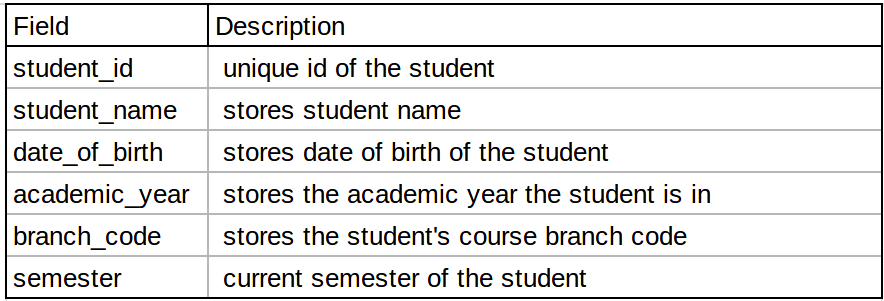
\includegraphics[scale=.5]{./StudentTable.png}
\\[0.2in]
\label{fig:Student Table}
\end{figure}
Since one teacher can teach many students, We thought it only right to insert a foreign key
branch\_code and semester into the student table. In addition, we have made the teacher account to have admin privilege. This will
enable us to focus more on the programming than on particulars of the database.\\
\pagebreak
\thispagestyle{fancy}
\section{Identify Major entities, attributes and relationships}
\begin{itemize}
\item Login page to give access to priviledged teachers.
\item Adding student and teacher details by the teacher.
\item Changing the id and password of the teacher.
which stores the details of transaction.
\item Teachers can check all details butnot passwords and modify them.
\item Teacher can delete the entities in the tables.
\item Easy  search facilities to get the reqiured information.
\end{itemize}

\thispagestyle{fancy}

\section{ER Schema}
\begin{figure}[H]
\centering
\caption{Entity Relationship Diagram}
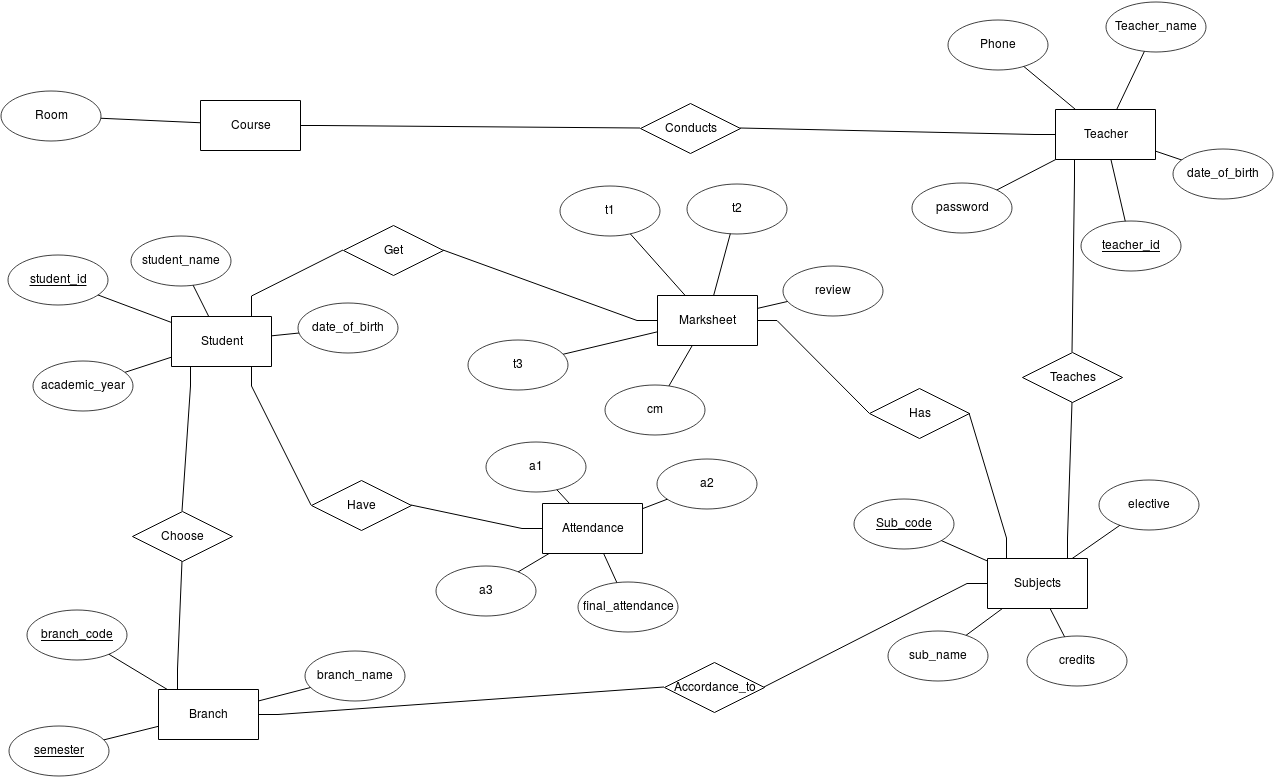
\includegraphics[width=\textwidth,height=\textheight,keepaspectratio]{./erd.png}
\\[0.2in]
\label{fig:Entitiy Relationship Diagram}
\end{figure}

\pagebreak
\thispagestyle{fancy}

\section{Schema Diagram}
\begin{figure}[H]
\centering
\caption{Relational Schema}
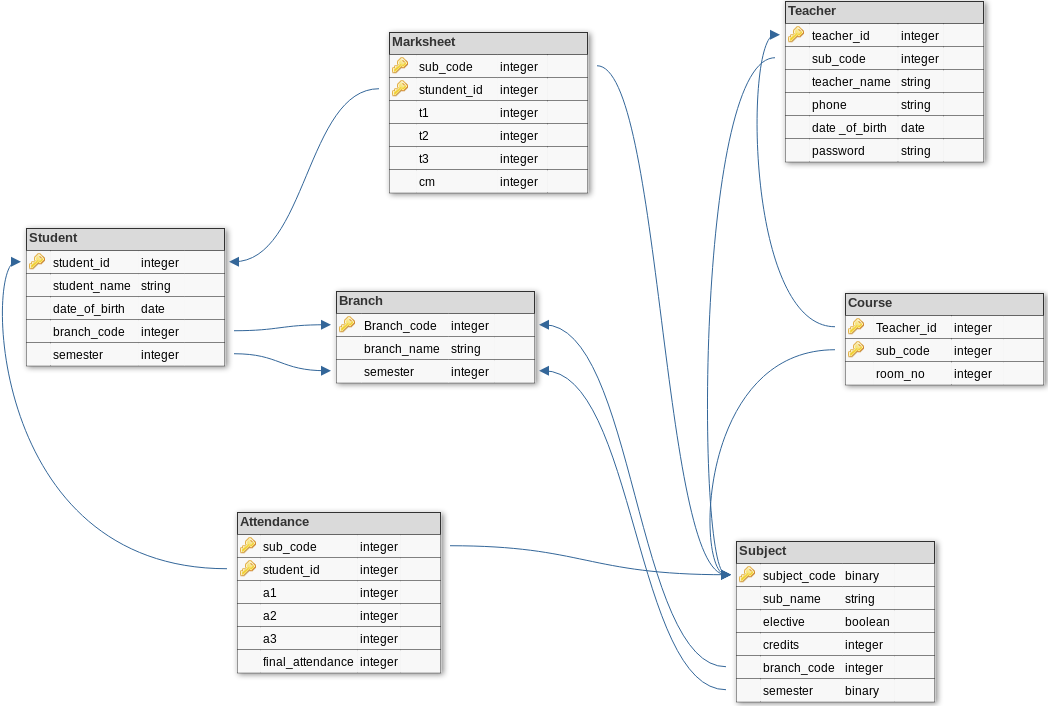
\includegraphics[scale=.5]{./schema.png}
\\[0.2in]
\label{fig:Relational Schema}
\end{figure}

\thispagestyle{fancy}
\chapter{Description Of Tools And Technologies}

\section{HTML}
Hypertext Markup Language (HTML) is the standard markup language for creating web pages and web applications. With Cascading Style Sheets (CSS) and JavaScript it forms a triad of cornerstone technologies for the World Wide Web. Web browsers receive HTML documents from a web server or from local storage and render them into multimedia web pages. HTML describes the structure of a web page semantically and originally included cues for the appearance of the document.
HTML elements are the building blocks of HTML pages. With HTML constructs, images and other objects, such as interactive forms, may be embedded into the rendered page. It provides a means to create structured documents by denoting structural semantics for text such as headings, paragraphs, lists, links, quotes and other items. HTML elements are delineated by tags, written using angle brackets. Tags such as <img /> and <input /> introduce content into the page directly. Others such as <p>...</p> surround and provide information about document text and may include other tags as sub-elements. Browsers do not display the HTML tags, but use them to interpret the content of the page.
HTML can embed programs written in a scripting language such as JavaScript which affect the behavior and content of web pages. Inclusion of CSS defines the look and layout of content. 

\section{Bootstrap - A CSS Framework}
Cascading Style Sheets (CSS) is a style sheet language used for describing the presentation of a document written in a markup language. Although most often used to set the visual style of web pages and user interfaces written in HTML and XHTML, the language can be applied to any XML document, including plain XML, SVG and XUL, and is applicable to rendering in speech, or on other media. Along with HTML and JavaScript, CSS is a cornerstone technology used by most websites to create visually engaging webpages, user interfaces for web applications, and user interfaces for many mobile applications.

CSS is designed primarily to enable the separation of presentation and content, including aspects such as the layout, colors, and fonts. This separation can improve content accessibility, provide more flexibility and control in the specification of presentation characteristics, enable multiple HTML pages to share formatting by specifying the relevant CSS in a separate .css file, and reduce complexity and repetition in the structural content.

Bootstrap is a free and open-source front-end web framework used for  designing websites and web applications. It contains HTML- and CSS-based design templates for typography, forms, buttons, navigation and other interface components, as well as optional JavaScript extensions. Unlike many web frameworks, it concerns itself with front-end development only.

Bootstrap is the second most-starred project on GitHub, with more than 111,600 stars and 51,500 forks.
\section{Javascript}
JavaScript, often abbreviated as JS, is a high-level, interpreted programming language. It is a language which is also characterized as dynamic, weakly typed, prototype-based and multi-paradigm.

Alongside HTML and CSS, JavaScript is one of the three core technologies of the World Wide Web. JavaScript enables interactive web pages and this is an essential part of web applications. The vast majority of websites use it, and all major web browsers have a dedicated JavaScript engine to execute it.

As a multi-paradigm language, JavaScript supports event-driven, functional, and imperative (including object-oriented and prototype-based) programming styles. It has an API for working with text, arrays, dates, regular expressions, and basic manipulation of the DOM, but the language itself does not include any I/O, such as networking, storage, or graphics facilities, relying for these upon the host environment in which it is embedded.

Initially only implemented client-side in web browsers, JavaScript engines are now embedded in many other types of host software, including server-side in web servers and databases, and in non-web programs such as word processors and PDF software, and in runtime environments that make JavaScript available for writing mobile and desktop applications, including desktop widgets.

Although there are strong outward similarities between JavaScript and Java, including language name, syntax, and respective standard libraries, the two languages are distinct and differ greatly in design; JavaScript was influenced by programming languages such as Self and Scheme.

\section{Python}
Python is an interpreted high-level programming language for general-purpose programming. Created by Guido van Rossum and first released in 1991, Python has a design philosophy that emphasizes code readability, notably using significant whitespace. It provides constructs that enable clear programming on both small and large scales. In July 2018, Van Rossum stepped down as the leader in the language community after 30 years.

Python features a dynamic type system and automatic memory management. It supports multiple programming paradigms, including object-oriented, imperative, functional and procedural, and has a large and comprehensive standard library.

Python interpreters are available for many operating systems. CPython, the reference implementation of Python, is open source software and has a community-based development model, as do nearly all of Python's other implementations. Python and CPython are managed by the non-profit Python Software Foundation. 


\section{SQLite}
SQLite is a relational database management system contained in a C programming library. In contrast to many other database management systems, SQLite is not a client–server database engine. Rather, it is embedded into the end program.SQLite is ACID-compliant and implements most of the SQL standard, using a dynamically and weakly typed SQL syntax that does not guarantee the domain integrity.SQLite is a popular choice as embedded database software for local/client storage in application software such as web browsers. It is arguably the most widely deployed database engine, as it is used today by several widespread browsers, operating systems, and embedded systems (such as mobile phones), among others.SQLite has bindings to many programming languages.
Unlike client–server database management systems, the SQLite engine has no standalone processes with which the application program communicates. Instead, the SQLite library is linked in and thus becomes an integral part of the application program. The library can also be called dynamically. The application program uses SQLite's functionality through simple function calls, which reduce latency in database access: function calls within a single process are more efficient than inter-process communication. SQLite stores the entire database (definitions, tables, indices, and the data itself) as a single cross-platform file on a host machine. It implements this simple design by locking the entire database file during writing. SQLite read operations can be multitasked, though writes can only be performed sequentially.
SQLite implements most of the SQL-92 standard for SQL but it lacks some features. For example, it partially provides triggers, and it can't write to views (however it provides INSTEAD OF triggers that provide this functionality). While it provides complex queries, it still has limited ALTER TABLE function, as it can't modify or delete columns.SQLite uses an unusual type system for an SQL-compatible DBMS; instead of assigning a type to a column as in most SQL database systems, types are assigned to individual values; in language terms it is dynamically typed. Moreover, it is weakly typed in some of the same ways that Perl is: one can insert a string into an integercolumn (although SQLite will try to convert the string to an integer first, if the column's preferred type is integer). This adds flexibility to columns, especially when bound to a dynamically typed scripting language. However, the technique is not portable to other SQL products. The SQLite web site describes a "strict affinity" mode, but this feature has not yet been added.[11] However, it can be implemented with constraints like CHECK(typeof(x)='integer').



\chapter{Results, Snapshots and Discussions}

\section{Section 1}
Lorem ipsum dolor sit amet, consectetur adipiscing elit. Aliquam luctus gravida odio nec sodales. Vivamus at sollicitudin dolor. Curabitur a quam eu tortor elementum consectetur. Fusce eget velit enim. Lorem ipsum dolor sit amet, consectetur adipiscing elit. Interdum et malesuada fames ac ante ipsum primis in faucibus. Praesent sed sagittis enim. Integer in tempus tellus. Donec accumsan est at ante pellentesque, eu dapibus nisi convallis. Pellentesque semper orci eget nulla scelerisque fermentum. Aenean vel feugiat tortor.

\thispagestyle{fancy}

\section{Section 2}
Lorem ipsum dolor sit amet, consectetur adipiscing elit. Aliquam luctus gravida odio nec sodales. Vivamus at sollicitudin dolor. Curabitur a quam eu tortor elementum consectetur. Fusce eget velit enim. Lorem ipsum dolor sit amet, consectetur adipiscing elit. Interdum et malesuada fames ac ante ipsum primis in faucibus. Praesent sed sagittis enim. Integer in tempus tellus. Donec accumsan est at ante pellentesque, eu dapibus nisi convallis. Pellentesque semper orci eget nulla scelerisque fermentum. Aenean vel feugiat tortor.

\thispagestyle{fancy}

\section{Section 3}
Lorem ipsum dolor sit amet, consectetur adipiscing elit. Aliquam luctus gravida odio nec sodales. Vivamus at sollicitudin dolor. Curabitur a quam eu tortor elementum consectetur. Fusce eget velit enim. Lorem ipsum dolor sit amet, consectetur adipiscing elit. Interdum et malesuada fames ac ante ipsum primis in faucibus. Praesent sed sagittis enim. Integer in tempus tellus. Donec accumsan est at ante pellentesque, eu dapibus nisi convallis. Pellentesque semper orci eget nulla scelerisque fermentum. Aenean vel feugiat tortor.

\thispagestyle{fancy}

\section{Section 4}
Lorem ipsum dolor sit amet, consectetur adipiscing elit. Aliquam luctus gravida odio nec sodales. Vivamus at sollicitudin dolor. Curabitur a quam eu tortor elementum consectetur. Fusce eget velit enim. Lorem ipsum dolor sit amet, consectetur adipiscing elit. Interdum et malesuada fames ac ante ipsum primis in faucibus. Praesent sed sagittis enim. Integer in tempus tellus. Donec accumsan est at ante pellentesque, eu dapibus nisi convallis. Pellentesque semper orci eget nulla scelerisque fermentum. Aenean vel feugiat tortor.

\thispagestyle{fancy}
\chapter{Conclusion and Future Enhancements}
This project is developed to nurture the needs of a user in a banking sector by embedding all
the tasks of transactions taking place in a bank. Future version of this project will still be
much enhanced than the current version. Writing and depositing checks are perhaps the most
fundamental ways to move money in and out of a checking account, but advancements in
technology have added ATM and debit card transactions. All banks have rules about how
long it takes to access your deposits, how many debit card transactions you're allowed in a
day, and how much cash you can withdraw from an ATM. Access to the balance in your
checking account can also be limited by businesses that place holds \\[0.2in]

The Banking Online System is a big and ambitious project. I am thankful for being
provided this great opportunity to work on it. As already mentioned, this project has gone
through extensive research work. On the basis of the research work, we have successfully
designed and implemented banking online System. To know what the future of online
banking looks like, its probably worth looking at the present online banking isnt new. When
you think of online banking, you probably think about a computer (either a desktop or
laptop), a three or four step security process and then an interface that lets you view the
balance of your various bank accounts and credit cards, whilst permitting you to transfer
money and pay bills. And youre not wrong either. \\[0.2in]
The most valuable future looks are following below:
\begin{itemize}
\item More branches of the bank, maybe it will be international, that means more ATM
machines outside.
\item Customer issues development based on their needs, so the help desk will be aware of
their needs and easy to use.
\item Developing a mobile App for banking system that help users to do the obtained his
operations without go to the bank only he need to sign in using his A/C NO. And
password and then use your own PIN. Finaly the system will update automatically.
\end{itemize}

\cleardoublepage
%\pagebreak
\phantomsection

\begin{thebibliography}{99}

\bibitem{}Fundamentals of database systems by (Elmasri Navathe, 2000)\\
Article: Online banking: \url{https://en.wikipedia.org/wiki/Online_banking}

\bibitem{} Online Bank Account Management System: \url{http://www.slideshare.net}

\bibitem{} Learning MYSQL, JavaScript, jQuery, JAVA : \url{http://www.w3schools.com}\\
PHP and MySQL video tutorials : \url{http://www.freebanglatutorial.com}, \url{http://www.youtube.com}

\bibitem{} Veneeva, V. (2006), E-Banking (Online Banking) and Its Role in Today's Society,
Ezine articles

\bibitem{} JavaScript validation for empty input field, \url{http://stackoverflow.com/questions/3937513/javascript-validation-for-e mptyinput-field}

\bibitem{} JavaScript form validation: Validate Password, Validate Email, Validate Phone
Number, \url{http://webcheatsheet.com/javascript/form_validation.php}
\end{thebibliography}



\end{document}


